\documentclass{exam}

\usepackage[table,x11names]{xcolor}
\usepackage{graphicx}
\usepackage{hyperref}

% Header and footer.
\pagestyle{headandfoot}
\runningheadrule
\runningfootrule
\runningfooter{}{Page \thepage\ of \numpages}{}
\firstpageheader{}{}{}

\printanswers

\title{\textbf{\tt Habib University}\\ \textbf{\tt CS 416 Algorithms for Machine Learning}\\ \textbf{\tt Fall 2018}}
\author{\textbf{\tt Emad Bin Abid}\\ {\tt $ea02893$}}
\date{\textbf{\tt Assignment 02}\\ \textbf{\tt Analysis Report} \\\textbf{\tt Submitted: October 12\textsuperscript{th}, 2018}}

\begin{document}
\maketitle

This report contains the visual + descriptive  analysis of the autoencoder architecture trained in the attached $.ipnb$ file.

\section{2-2 Conv-Conv Design:}
	This design has 2 encoder and 2 decoder layers. The analysis is divided into three parts:

	\begin{description}
		\item[$\cdot$] Effect of varying LR on constant batch size and epoch.
		\item[$\cdot$] Effect of varying batch size on constant LR and epoch.
		\item[$\cdot$] Effect of varying epoch on constant LR and batch size.
	\end{description}
\pagebreak

	\subsection{Varying LR:}
		\begin{description}
			\item[$\cdot$] Batch size = 32 and Epochs = 10.		
		\end{description}			

		\begin{table}[h!]
  			\begin{center}
    			\caption{}
    			\begin{tabular}{l|l|l|r|r|r}
      				\textbf{Epoch} & \textbf{M.S.E. @ LR=0.1} & \textbf{M.S.E. @ LR=0.01} & \textbf{M.S.E. @ LR=0.001} & \textbf{M.S.E. @ LR=0.0001}\\
      				\hline
      				\rowcolor{pink} 1 & 0.005940 & 0.008400 & 0.014045 & 0.045864 \\
      				2 & 0.004542 & 0.006082 & 0.008670 & 0.017278 \\
      				3 & 0.004184 & 0.005550 & 0.007915 & 0.013715 \\
      				4 & 0.003933 & 0.005290 & 0.007434 & 0.012317 \\
      				5 & 0.003759 & 0.005113 & 0.007090 & 0.011503 \\
      				6 & 0.003614 & 0.004989 & 0.006821 & 0.010939 \\
      				7 & 0.003496 & 0.004879 & 0.006613 & 0.010531 \\
      				8 & 0.003392 & 0.004793 & 0.006440 & 0.010204 \\
      				9 & 0.003308 & 0.004709 & 0.006283 & 0.009932 \\
      				\rowcolor{yellow} 10 & 0.003232 & 0.004640 & 0.006153 & 0.009696 \\
      				 & 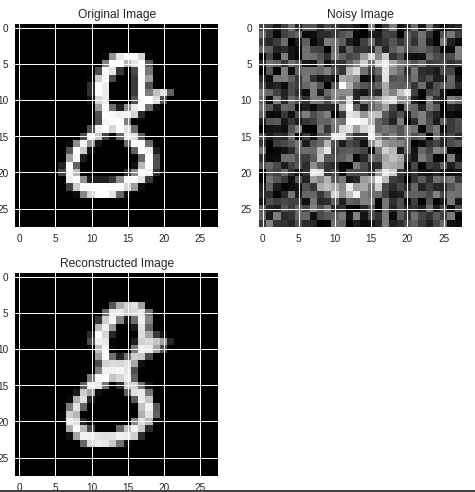
\includegraphics[scale=0.3]{../assets/1.png} & 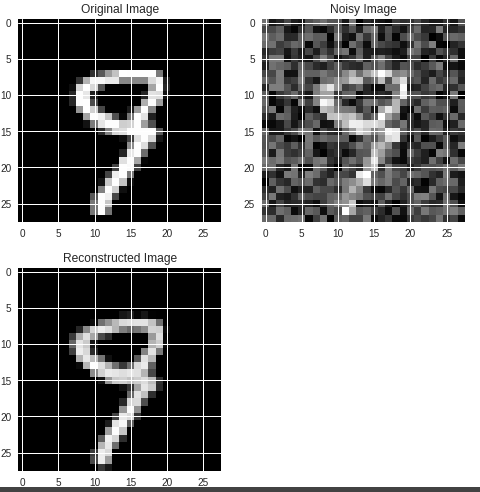
\includegraphics[scale=0.3]{../assets/2.png} & 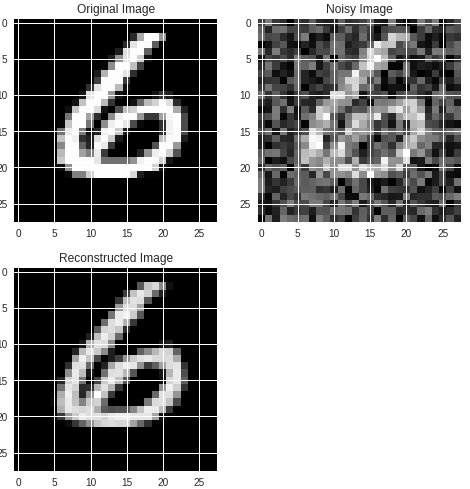
\includegraphics[scale=0.3]{../assets/3.png} & 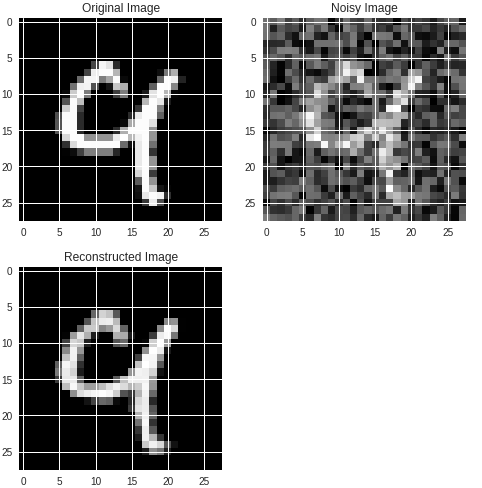
\includegraphics[scale=0.3]{../assets/4.png}
    			\end{tabular}
  			\end{center}
		\end{table}			
\pagebreak	
			
\subsection{Varying Batch Size:}
		\begin{description}
			\item[$\cdot$] LR = 0.1 and Epochs = 10.		
		\end{description}			

		\begin{table}[h!]
  			\begin{center}
    			\caption{}
    			\begin{tabular}{l|l|l|r|r|r}
      				\textbf{Epoch} & \textbf{M.S.E. @ BS=16} & \textbf{M.S.E. @ BS=32} & \textbf{M.S.E. @ BS=64} & \textbf{M.S.E. @ BS=128}\\
      				\hline
      				\rowcolor{pink} 1 & 0.005940 & 0.008400 & 0.014045 & 0.045864 \\
      				2 & 0.004542 & 0.006082 & 0.008670 & 0.017278 \\
      				3 & 0.004184 & 0.005550 & 0.007915 & 0.013715 \\
      				4 & 0.003933 & 0.005290 & 0.007434 & 0.012317 \\
      				5 & 0.003759 & 0.005113 & 0.007090 & 0.011503 \\
      				6 & 0.003614 & 0.004989 & 0.006821 & 0.010939 \\
      				7 & 0.003496 & 0.004879 & 0.006613 & 0.010531 \\
      				8 & 0.003392 & 0.004793 & 0.006440 & 0.010204 \\
      				9 & 0.003308 & 0.004709 & 0.006283 & 0.009932 \\
      				\rowcolor{yellow} 10 & 0.003232 & 0.004640 & 0.006153 & 0.009696 \\
      				& 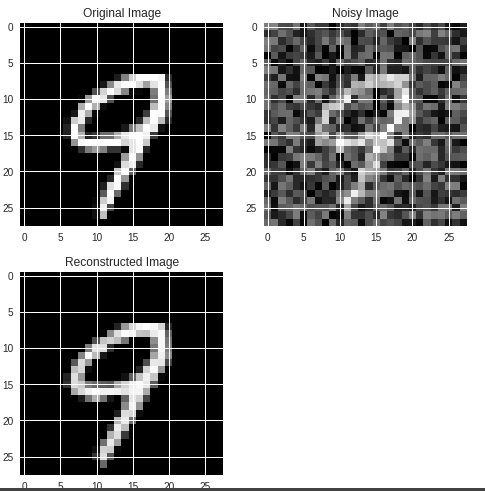
\includegraphics[scale=0.3]{../assets/5.png} & 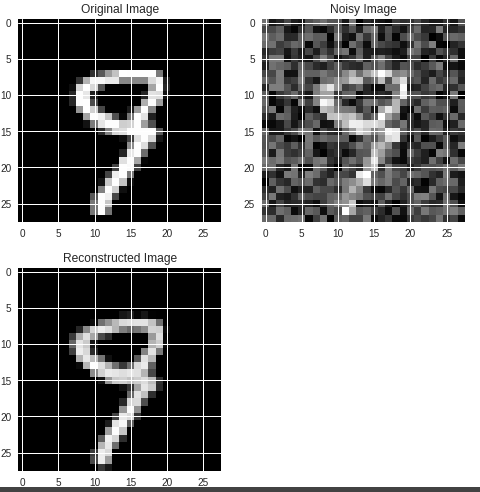
\includegraphics[scale=0.3]{../assets/6.png} & 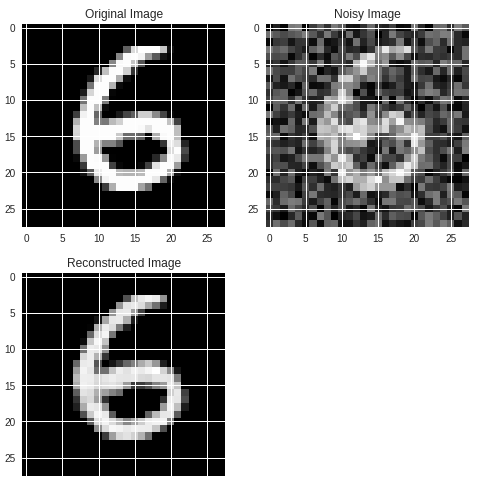
\includegraphics[scale=0.3]{../assets/7.png} & 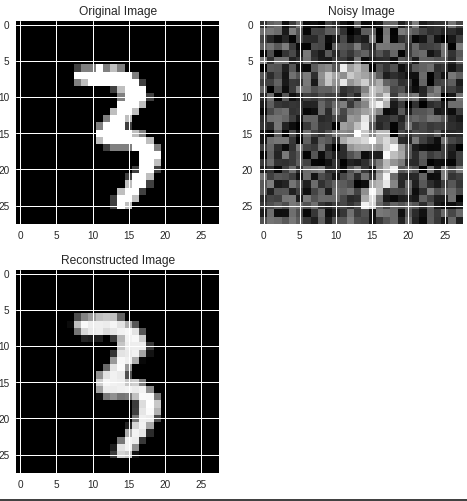
\includegraphics[scale=0.3]{../assets/8.png}
    			\end{tabular}
  			\end{center}
		\end{table}
\pagebreak	
	
\subsection{Varying Epochs:}
		\begin{description}
			\item[$\cdot$] LR = 0.1 and Batch Size = 32.		
		\end{description}			

		\begin{table}[h!]
  			\begin{center}
    			\caption{}
    			\begin{tabular}{l|l|l|r|r|r}
      				\textbf{Epoch} & \textbf{M.S.E. @ Epoch=10} & \textbf{M.S.E. @ BS=100} & \textbf{M.S.E. @ BS=500}\\
      				\hline
      				\rowcolor{pink} 1 & 0.005940 & 0. & 0.\\
      								2 & 0.004542 & 0. & 0.\\
      								3 & 0.004184 & 0. & 0.\\
      								4 & 0.003933 & 0. & 0.\\
      								5 & 0.003759 & 0. & 0.\\
      								6 & 0.003614 & 0. & 0.\\
      								7 & 0.003496 & 0. & 0.\\
      								8 & 0.003392 & 0. & 0.\\
      								9 & 0.003308 & 0. & 0.\\
      			  \rowcolor{yellow} 10 & 0.003232 & 0. & 0.\\
      			   & 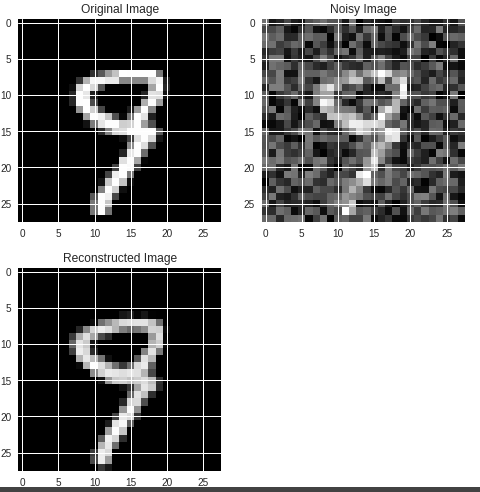
\includegraphics[scale=0.3]{../assets/9.png} &  & \\
      			  					... &  & ... & ... \\
      			  \rowcolor{yellow} 100 &  & 0.002229 & 0.002193 \\
      			  &   & 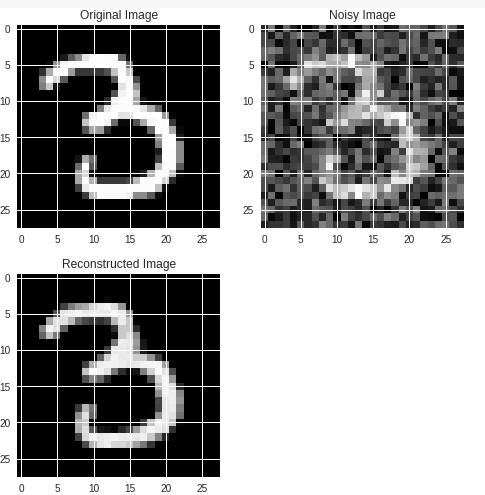
\includegraphics[scale=0.3]{../assets/10.png}  & \\
      			  					... &  &  & ... \\
      			  \rowcolor{yellow} 500 &  &  & 0.001136 \\
      			  &  &  & 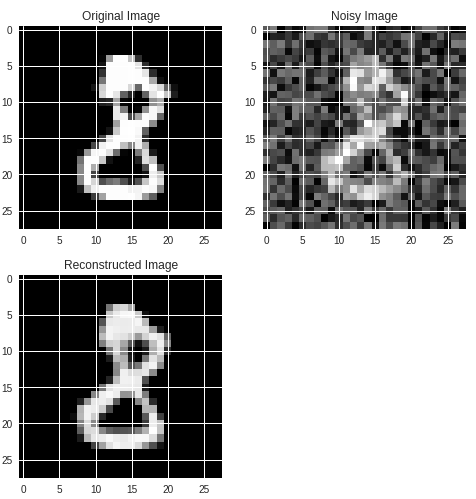
\includegraphics[scale=0.3]{../assets/11.png}\\	  						  					
    			\end{tabular}
  			\end{center}
		\end{table}
		
The trained architecture is inspired from \href{https://github.com/GunhoChoi/Kind-PyTorch-Tutorial/blob/master/07_Denoising_Autoencoder/Denoising_Autoencoder.py}{\underline{here}}.
\end{document}